%% bare_conf.tex
%% V1.4b
%% 2015/08/26
%% by Michael Shell
%% See:
%% http://www.michaelshell.org/
%% for current contact information.
%%
%% This is a skeleton file demonstrating the use of IEEEtran.cls
%% (requires IEEEtran.cls version 1.8b or later) with an IEEE
%% conference paper.
%%
%% Support sites:
%% http://www.michaelshell.org/tex/ieeetran/
%% http://www.ctan.org/pkg/ieeetran
%% and
%% http://www.ieee.org/

%%*************************************************************************
%% Legal Notice:
%% This code is offered as-is without any warranty either expressed or
%% implied; without even the implied warranty of MERCHANTABILITY or
%% FITNESS FOR A PARTICULAR PURPOSE! 
%% User assumes all risk.
%% In no event shall the IEEE or any contributor to this code be liable for
%% any damages or losses, including, but not limited to, incidental,
%% consequential, or any other damages, resulting from the use or misuse
%% of any information contained here.
%%
%% All comments are the opinions of their respective authors and are not
%% necessarily endorsed by the IEEE.
%%
%% This work is distributed under the LaTeX Project Public License (LPPL)
%% ( http://www.latex-project.org/ ) version 1.3, and may be freely used,
%% distributed and modified. A copy of the LPPL, version 1.3, is included
%% in the base LaTeX documentation of all distributions of LaTeX released
%% 2003/12/01 or later.
%% Retain all contribution notices and credits.
%% ** Modified files should be clearly indicated as such, including  **
%% ** renaming them and changing author support contact information. **
%%*************************************************************************


% *** Authors should verify (and, if needed, correct) their LaTeX system  ***
% *** with the testflow diagnostic prior to trusting their LaTeX platform ***
% *** with production work. The IEEE's font choices and paper sizes can   ***
% *** trigger bugs that do not appear when using other class files.       ***                          ***
% The testflow support page is at:
% http://www.michaelshell.org/tex/testflow/



\documentclass[conference]{IEEEtran}
% Some Computer Society conferences also require the compsoc mode option,
% but others use the standard conference format.
%
% If IEEEtran.cls has not been installed into the LaTeX system files,
% manually specify the path to it like:
% \documentclass[conference]{../sty/IEEEtran}





% Some very useful LaTeX packages include:
% (uncomment the ones you want to load)


% *** MISC UTILITY PACKAGES ***
%
%\usepackage{ifpdf}
% Heiko Oberdiek's ifpdf.sty is very useful if you need conditional
% compilation based on whether the output is pdf or dvi.
% usage:
% \ifpdf
%   % pdf code
% \else
%   % dvi code
% \fi
% The latest version of ifpdf.sty can be obtained from:
% http://www.ctan.org/pkg/ifpdf
% Also, note that IEEEtran.cls V1.7 and later provides a builtin
% \ifCLASSINFOpdf conditional that works the same way.
% When switching from latex to pdflatex and vice-versa, the compiler may
% have to be run twice to clear warning/error messages.


% *** CITATION PACKAGES ***
%
\usepackage{cite}
% cite.sty was written by Donald Arseneau
% V1.6 and later of IEEEtran pre-defines the format of the cite.sty package
% \cite{} output to follow that of the IEEE. Loading the cite package will
% result in citation numbers being automatically sorted and properly
% "compressed/ranged". e.g., [1], [9], [2], [7], [5], [6] without using
% cite.sty will become [1], [2], [5]--[7], [9] using cite.sty. cite.sty's
% \cite will automatically add leading space, if needed. Use cite.sty's
% noadjust option (cite.sty V3.8 and later) if you want to turn this off
% such as if a citation ever needs to be enclosed in parenthesis.
% cite.sty is already installed on most LaTeX systems. Be sure and use
% version 5.0 (2009-03-20) and later if using hyperref.sty.
% The latest version can be obtained at:
% http://www.ctan.org/pkg/cite
% The documentation is contained in the cite.sty file itself.


% *** GRAPHICS RELATED PACKAGES ***
%
\ifCLASSINFOpdf
\usepackage[pdftex]{graphicx}
  % declare the path(s) where your graphic files are
  % \graphicspath{{../pdf/}{../jpeg/}}
  % and their extensions so you won't have to specify these with
  % every instance of \includegraphics
  % \DeclareGraphicsExtensions{.pdf,.jpeg,.png}
\else
  % or other class option (dvipsone, dvipdf, if not using dvips). graphicx
  % will default to the driver specified in the system graphics.cfg if no
  % driver is specified.
  % \usepackage[dvips]{graphicx}
  % declare the path(s) where your graphic files are
  % \graphicspath{{../eps/}}
  % and their extensions so you won't have to specify these with
  % every instance of \includegraphics
  % \DeclareGraphicsExtensions{.eps}
\fi
% graphicx was written by David Carlisle and Sebastian Rahtz. It is
% required if you want graphics, photos, etc. graphicx.sty is already
% installed on most LaTeX systems. The latest version and documentation
% can be obtained at: 
% http://www.ctan.org/pkg/graphicx
% Another good source of documentation is "Using Imported Graphics in
% LaTeX2e" by Keith Reckdahl which can be found at:
% http://www.ctan.org/pkg/epslatex
%
% latex, and pdflatex in dvi mode, support graphics in encapsulated
% postscript (.eps) format. pdflatex in pdf mode supports graphics
% in .pdf, .jpeg, .png and .mps (metapost) formats. Users should ensure
% that all non-photo figures use a vector format (.eps, .pdf, .mps) and
% not a bitmapped formats (.jpeg, .png). The IEEE frowns on bitmapped formats
% which can result in "jaggedy"/blurry rendering of lines and letters as
% well as large increases in file sizes.
%
% You can find documentation about the pdfTeX application at:
% http://www.tug.org/applications/pdftex

% *** MATH PACKAGES ***
%
%\usepackage{amsmath}
% A popular package from the American Mathematical Society that provides
% many useful and powerful commands for dealing with mathematics.
%
% Note that the amsmath package sets \interdisplaylinepenalty to 10000
% thus preventing page breaks from occurring within multiline equations. Use:
%\interdisplaylinepenalty=2500
% after loading amsmath to restore such page breaks as IEEEtran.cls normally
% does. amsmath.sty is already installed on most LaTeX systems. The latest
% version and documentation can be obtained at:
% http://www.ctan.org/pkg/amsmath

% *** SPECIALIZED LIST PACKAGES ***
%
\usepackage{algorithm}
\usepackage{algpseudocode}
% algorithmic.sty was written by Peter Williams and Rogerio Brito.
% This package provides an algorithmic environment fo describing algorithms.
% You can use the algorithmic environment in-text or within a figure
% environment to provide for a floating algorithm. Do NOT use the algorithm
% floating environment provided by algorithm.sty (by the same authors) or
% algorithm2e.sty (by Christophe Fiorio) as the IEEE does not use dedicated
% algorithm float types and packages that provide these will not provide
% correct IEEE style captions. The latest version and documentation of
% algorithmic.sty can be obtained at:
% http://www.ctan.org/pkg/algorithms
% Also of interest may be the (relatively newer and more customizable)
% algorithmicx.sty package by Szasz Janos:
% http://www.ctan.org/pkg/algorithmicx

% *** ALIGNMENT PACKAGES ***
%
%\usepackage{array}
% Frank Mittelbach's and David Carlisle's array.sty patches and improves
% the standard LaTeX2e array and tabular environments to provide better
% appearance and additional user controls. As the default LaTeX2e table
% generation code is lacking to the point of almost being broken with
% respect to the quality of the end results, all users are strongly
% advised to use an enhanced (at the very least that provided by array.sty)
% set of table tools. array.sty is already installed on most systems. The
% latest version and documentation can be obtained at:
% http://www.ctan.org/pkg/array


% IEEEtran contains the IEEEeqnarray family of commands that can be used to
% generate multiline equations as well as matrices, tables, etc., of high
% quality.


% *** SUBFIGURE PACKAGES ***
%\ifCLASSOPTIONcompsoc
%  \usepackage[caption=false,font=normalsize,labelfont=sf,textfont=sf]{subfig}
%\else
%  \usepackage[caption=false,font=footnotesize]{subfig}
%\fi
% subfig.sty, written by Steven Douglas Cochran, is the modern replacement
% for subfigure.sty, the latter of which is no longer maintained and is
% incompatible with some LaTeX packages including fixltx2e. However,
% subfig.sty requires and automatically loads Axel Sommerfeldt's caption.sty
% which will override IEEEtran.cls' handling of captions and this will result
% in non-IEEE style figure/table captions. To prevent this problem, be sure
% and invoke subfig.sty's "caption=false" package option (available since
% subfig.sty version 1.3, 2005/06/28) as this is will preserve IEEEtran.cls
% handling of captions.
% Note that the Computer Society format requires a larger sans serif font
% than the serif footnote size font used in traditional IEEE formatting
% and thus the need to invoke different subfig.sty package options depending
% on whether compsoc mode has been enabled.
%
% The latest version and documentation of subfig.sty can be obtained at:
% http://www.ctan.org/pkg/subfig




% *** FLOAT PACKAGES ***
%
%\usepackage{fixltx2e}
% fixltx2e, the successor to the earlier fix2col.sty, was written by
% Frank Mittelbach and David Carlisle. This package corrects a few problems
% in the LaTeX2e kernel, the most notable of which is that in current
% LaTeX2e releases, the ordering of single and double column floats is not
% guaranteed to be preserved. Thus, an unpatched LaTeX2e can allow a
% single column figure to be placed prior to an earlier double column
% figure.
% Be aware that LaTeX2e kernels dated 2015 and later have fixltx2e.sty's
% corrections already built into the system in which case a warning will
% be issued if an attempt is made to load fixltx2e.sty as it is no longer
% needed.
% The latest version and documentation can be found at:
% http://www.ctan.org/pkg/fixltx2e


%\usepackage{stfloats}
% stfloats.sty was written by Sigitas Tolusis. This package gives LaTeX2e
% the ability to do double column floats at the bottom of the page as well
% as the top. (e.g., "\begin{figure*}[!b]" is not normally possible in
% LaTeX2e). It also provides a command:
%\fnbelowfloat
% to enable the placement of footnotes below bottom floats (the standard
% LaTeX2e kernel puts them above bottom floats). This is an invasive package
% which rewrites many portions of the LaTeX2e float routines. It may not work
% with other packages that modify the LaTeX2e float routines. The latest
% version and documentation can be obtained at:
% http://www.ctan.org/pkg/stfloats
% Do not use the stfloats baselinefloat ability as the IEEE does not allow
% \baselineskip to stretch. Authors submitting work to the IEEE should note
% that the IEEE rarely uses double column equations and that authors should try
% to avoid such use. Do not be tempted to use the cuted.sty or midfloat.sty
% packages (also by Sigitas Tolusis) as the IEEE does not format its papers in
% such ways.
% Do not attempt to use stfloats with fixltx2e as they are incompatible.
% Instead, use Morten Hogholm'a dblfloatfix which combines the features
% of both fixltx2e and stfloats:
%
% \usepackage{dblfloatfix}
% The latest version can be found at:
% http://www.ctan.org/pkg/dblfloatfix

% *** PDF, URL AND HYPERLINK PACKAGES ***
%
\usepackage{url}
% url.sty was written by Donald Arseneau. It provides better support for
% handling and breaking URLs. url.sty is already installed on most LaTeX
% systems. The latest version and documentation can be obtained at:
% http://www.ctan.org/pkg/url
% Basically, \url{my_url_here}.




% *** Do not adjust lengths that control margins, column widths, etc. ***
% *** Do not use packages that alter fonts (such as pslatex).         ***
% There should be no need to do such things with IEEEtran.cls V1.6 and later.
% (Unless specifically asked to do so by the journal or conference you plan
% to submit to, of course. )


% correct bad hyphenation here
\hyphenation{op-tical net-works semi-conduc-tor}


\begin{document}
%
% paper title
% Titles are generally capitalized except for words such as a, an, and, as,
% at, but, by, for, in, nor, of, on, or, the, to and up, which are usually
% not capitalized unless they are the first or last word of the title.
% Linebreaks \\ can be used within to get better formatting as desired.
% Do not put math or special symbols in the title.
\title{Rapid detection of disobedient forwarding on a compromised OpenFlow switch}


% author names and affiliations
% use a multiple column layout for up to three different
% affiliations
\author{\IEEEauthorblockN{Yen-Chun Chiu, Po-Ching Lin}
\IEEEauthorblockA{Department of Computer Science and\\Information Engineering\\
National Chung Cheng University\\
Chiayi, Taiwan 62102\\
Email: shuaichiou@gmail.com, pclin@cs.ccu.edu.tw}}

% conference papers do not typically use \thanks and this command
% is locked out in conference mode. If really needed, such as for
% the acknowledgment of grants, issue a \IEEEoverridecommandlockouts
% after \documentclass

% for over three affiliations, or if they all won't fit within the width
% of the page, use this alternative format:
% 
%\author{\IEEEauthorblockN{Michael Shell\IEEEauthorrefmark{1},
%Homer Simpson\IEEEauthorrefmark{2},
%James Kirk\IEEEauthorrefmark{3}, 
%Montgomery Scott\IEEEauthorrefmark{3} and
%Eldon Tyrell\IEEEauthorrefmark{4}}
%\IEEEauthorblockA{\IEEEauthorrefmark{1}School of Electrical and Computer Engineering\\
%Georgia Institute of Technology,
%Atlanta, Georgia 30332--0250\\ Email: see http://www.michaelshell.org/contact.html}
%\IEEEauthorblockA{\IEEEauthorrefmark{2}Twentieth Century Fox, Springfield, USA\\
%Email: homer@thesimpsons.com}
%\IEEEauthorblockA{\IEEEauthorrefmark{3}Starfleet Academy, San Francisco, California 96678-2391\\
%Telephone: (800) 555--1212, Fax: (888) 555--1212}
%\IEEEauthorblockA{\IEEEauthorrefmark{4}Tyrell Inc., 123 Replicant Street, Los Angeles, California 90210--4321}}

% use for special paper notices
%\IEEEspecialpapernotice{(Invited Paper)}

% make the title area
\maketitle

% As a general rule, do not put math, special symbols or citations
% in the abstract
\begin{abstract}
Software-defined networking (SDN) is programmable, centrally managed, and flexible with topology alteration. It allows network administrators to manage network flows easily from a centralized controller. However, these new features also lead to new security threats with applications, controllers, OpenFlow switches, topology management and so on. We study the attack of compromising a switch, and design a method to detect disobedient forwarding in the flow table. To enhance the detection efficiency and minimize additional network traffic, we reduce the number of detection packets necessary by aggregating the flow entries in a short time. To aggregate the flow entries, we select entries whose match fields are able to compose a valid packet from different switches. The switches on which the entries are form a path that allows the packet to travel through for rapid detection. We evaluate the effectiveness of this detection method in various topology types typically found in a data center network by Mininet simulation. The experimental result demonstrates that this method can examine the forwarding correctness of nearly 3 flow entries simultaneously on average for each detection packet. Furthermore, since the positive and negative factors to the growth of aggregation rates break even in a large topology, the scale of the network topology does not affect the efficiency of the method significantly.
\end{abstract}

% no keywords
% For peer review papers, you can put extra information on the cover
% page as needed:
% \ifCLASSOPTIONpeerreview
% \begin{center} \bfseries EDICS Category: 3-BBND \end{center}
% \fi
%
% For peerreview papers, this IEEEtran command inserts a page break and
% creates the second title. It will be ignored for other modes.
\IEEEpeerreviewmaketitle

\section{Introduction}
\label{chap:intro}
Software-defined networking (SDN) is a dynamic, programmable, cost-effective solution that gains great popularity in the industry and academia in recent years. A controller can centrally manage the flow rules on the switches in a consistent manner, and network applications can be developed on the controller for flexible management. Nevertheless, SDN often comes with new security threats \cite{SOS13} as new mechanisms such as topology discovery, host management, OpenFlow protocols and application interfaces have been introduced. For example, applications may be malicious, topology discovery and host management mechanisms can be leveraged to launch man-in-the-middle or denial-of-service attacks, malicious controllers may affect the control channel, and switches and hosts may be compromised.

Since Openflow switches lie between the controller and the hosts, an attacker can utilize a number of components to perform attacks. In \cite{HXWG15}, Hong et al. studied the attacks that poison network visibility and its countermeasure, but the situation in which switches are compromised is not considered. Also, a compromised switch is able to modify its own flow entries for malicious behavior like undesired forwarding or packet dropping. It can also connect to a malicious controller and influence the network by manipulating the control traffic in the way the attacker desires, such as sending forged OpenFlow messages. Another type of attack is to exploit the topology discovery mechanism, making the controller into believing the existence of non-existing links.

Although some protection methods have been proposed \cite{CKGL15,PJL16}, there has not been an efficient way to detect if there is any compromised switch in SDN. The detection method in \cite{CKGL15} tests if a flow entry works as expected one at a time, which is inefficient in a large network. FADE presented in \cite{PJL16} results in some false negative results and takes a while to go through the entire network. ATPG in \cite{ZKVM12} is able to test through all the rules in the network with few packets in a short time. However, it is designed for regular networks in the Internet, deployment takes a lot of efforts such as setting up test terminals and network monitors. In our work, we present a method to discover compromised switches if they do not follow the flow rules, it reduces the cost of detecting compromised switches and speed up the entire detection process flexibly. We fabricate the detection packets so that each can test multiple flow entries on multiple switches at a time by exploiting identical match field values or exclusive match fields in the flow entries. 
The main contributions of this work are as follows:

\begin{enumerate}
\item
Analyze attacks related to flow entry manipulation, which influences the visibility of network.
\item
Discuss existing countermeasures to such attacks.
\item
Propose a switch entry validation method that verifies all the entries inside the network with aggregation technique.
\item
Evaluate the effectiveness of the method with various control variables.
\end{enumerate}

The following chapters are organized as follows. Section 2 gives detailed background knowledge of related technology and discusses possible threats and countermeasures. Section 3 is about the threat model and the theory behind the detection method. Section 4 contains the experimental details including setup, considerations and evaluation methods. Finally, the conclusion and future expectation of this work will be in Section 5.

\section{Background and related work}
\subsection{SDN and OpenFlow}
\label{SDN and OpenFlow}
OpenFlow is the most popular southbound interface in SDN. A switch that supports OpenFlow is called an OpenFlow switch. OpenFlow switches typically separate OpenFlow and non-OpenFlow traffic, which do not interfere with each other. There is usually a table-miss entry with the lowest priority and wildcards in all the match fields for handling the packets that cannot match any other flow entries[https://www.opennetworking.org/images/stories/downloads/sdn-resources/onfspecifications/openflow/openflow-switch-v1.5.1.pdf]. Usually, such a packet will be sent to the controller using the controller-reserved port, then the controller decides how to process it and adds a new entry according to the network policy. 

\subsection{Compromised OpenFlow switches}
\label{SDN security}
In this work, we will focus on the issue of compromised OpenFlow switches, since it has been less addressed than the others so far. Compromising OpenFlow switches can lead to some negative results: (1) Attackers may launch topology poisoning attack by manipulating link discovery packets. (2) The the flow entries on a compromised switch can be unexpectedly altered. (3) The packets that pass through a compromised switch can be eavesdropped or dropped. (4) The compromised switch may be configured to be managed by another malicious controller. (5) It is possible to launch network-wide denial-of-service attack by sending specific forged packets to consume the controller's resource. 

Unwanted flow entry modification on the compromised switch may lead to MITM, eavesdropping or DOS attack \cite{AAS14}. The detection method proposed in \cite{CKGL15} select a flow entry as the detecting target and install new entries on its neighbors. With the match field selected by their algorithm, every packet that matches the new flow entry will match the target flow entry. A packet containing the match field of the new flow entry will be sent from \texttt{Packet\_Out} to a neighbor of the target switch, forwarded to the target switch, go through the series of switches, and should be sent back to the controller. Finally, they will check if the packet comes back to the controller as expected and remains unchanged. However, this method will take a long time to run if it is desired to scan through a large number of flow entries. A pre-detection method to narrow down the potential targets is needed.

In \cite{PJL16}, Pang et al. design a method to detect the forwarding anomaly. First, they find a minimal set of flows whose rule paths cover all flows. Next, additional dedicated flow entries with timeout will be installed, the actions of these dedicated entries will modify the label, and a label will be added into packets to collect flow statistics. The more dedicated entries are used, the more likely they are able to identify where the malicious flow entry is located. However, if the dedicated rules are installed right on the malicious switch, the newly installed entry may be matched prior to the malicious entry and the method will not work. Therefore, they need to calculate the optimal number of dedicated entries to install to reach a balance between efficiency and probability to detect the malicious flow entries successfully. Their experimental result shows that FADE is able to detect forwarding anomaly in a network topology containing around 30 switches in 15 minutes with 2.5\% false negative and 4\% throughput reduction.

\subsection{Network debugging in SDN}
Some network debugging methods can be quite inspiring for the development of malicious behavior detection method. Flow entry information gathering techniques can also be found in \cite{ARDC14}. Just like traceroute, Agarwal et al. aim to trace the traveling path of a packet in an SDN network with minimal influence to the network. They use the VLAN field as color labels of switches and send the probing packets to the controller for logging or use the actual forwarding rules in the switch when receiving probing packets from the controller. When malicious behavior like packet dropping occurs, it is also likely to find the culprit by checking the last hop of the probing packet.

Automatic Test Packet Generation (ATPG) proposed in \cite{ZKVM12} is able to test through tremendous number of flow rules and links with the packets less than 1\% of the traffic in an automatic way. They keep a list of rule histories for each pair of ingress and egress port, find the minimal subset of test packets whose travel path covers the detection objective, and check if the actions are executed normally when packet reaches an end point. Since that work runs on regular networks, it requires deployment of terminals for generating test packets. In contrast, we use multiple action sets and deploy new flow entries to duplicate detection packets and send them to other switches in a tree-like manner. This increases the number of entries a single detection packet is able to detect. 

\section{Detection method}
This work focuses on the problem that a compromised switch will bring and presents the method to detect such a switch. Our method emphasizes on scanning through the whole network with fewer packets and high detection efficiency. In this chapter, we will define the threat models and how the problems can be solved with the presented detection algorithm.

\subsection{Threat models and Attack scenarios}
We assume the following scenarios of compromising a switch in the threat models:
\begin{enumerate}
\item
Only one OpenFlow switch is compromised. No cooperation among multiple compromised switches for attacks will happen.
\item
An attacker only perform the attack by modifying flow entries.
\item
Initially, the network is clean, and nothing is compromised. The attacks take place some time after the whole network is established.
\end{enumerate}

\subsection{Rapid detection method of disobedient forwarding}
Our method aims to detect if the flow entries of switches in the network work as expected. Our method has two main enhancements. First, it reduces the number of detection packets required, and therefore increases the efficiency significantly. Second, no existing flow entry is modified. Only some temporary entries will be added and will be timeout after the detection process is over, which has little influence to the whole network. 

Here are some terminologies used in our method:
\begin{description}
\item
Aggregation conditions: The conditions for an entry to be in the same aggregated group. They ensure a valid detection packet can be forged and sent successfully. The conditions are as follows:
\begin{enumerate}
\item
In the same group, the flow entries on different switches either have exactly the same match fields and values, or have no common match fields.
\item
A detection packet should not visit a switch more than once.
\item
A entry \textit{A} may only belong to more than one aggregated group if there exists another flow entry \textit{B} on another switch that \textit{A} and \textit{B} have the same match field and value.
\end{enumerate}

\item
Aggregated groups: A set of entries that satisfy the aggregation conditions.

\item 
Aggregation tree: A tree-formated structure representing the packet traversal path of a detection packet. It contains starting switch: the switch as a starting point for traversal, splitting switches, the switches which have more than one child and are responsible of duplicating the detection packet and sending them to the children and leaf switches, the switches which are the leaves of an aggregation tree.

\item
Detection packets: It is forged according to the match fields of the flow entries in an aggregated group. The VLAN identifier (vid) of each detection packet is set to the group identifier it is associated with.

\item 
Auxiliary entry: The entry that will be added to splitting switches to duplicate the detection packet or leaf switches to send the packet back to the controller.
\end{description}

\subsubsection{The detection method}
\label{Detection_method}

The main idea of the method is to assemble a packet and send it into the network. It goes through the switches, and should be sent back to the controller from expected switches finally if nothing goes wrong. Therefore, the detection packet can check whether the matched flow entries on these switches work as expected or not. For this purpose, we need to find the path that a detection packet should traverse, find the flow entries on each switch with which the packet will be matched, and set the fields in the packet so that it will pass through the switches in order. Because the controller has the network-wise visibility and the policy of all the flow entries, it is able to decide the switches to be involved in an aggregation tree and the detection packet in each run of detection. 

\begin{figure}[ht]
\centering
\includegraphics[width=1\linewidth]{figures/flow_entry_detection_flowchart.png}
\caption{The flow chart of the flow entry detection process.}
\label{flow_entry_detection_flowchart}
\end{figure}

The first aggregation condition allows us to forge a packet with multiple fields that matches the entries inside the same aggregated group. The second condition is to ensure the detection packet does not get stuck in a loop and never comes back to the controller. The third aggregation condition is also for eliminating loops, we will talk more about it in Section~\ref{Aggregated_group_finding}.

Since a detection packet is needed for each aggregated group, minimizing the number of aggregated groups results in fast detection. Hence, we try to increase the number of entries that one detection packet goes through. On a switch, there may be a collection of entries that fit the aggregation conditions. We can add an auxiliary flow entry with multiple forwarding actions that duplicate the detection packet and forward them to the switches on which the next entries in an aggregated group are.

As the abstraction of the problem, we treat switches as vertices and forwarding actions as edges. Our goal is to find the minimum number aggregated groups such that all the entries belong to at least an aggregated group. It forms a complex set covering problem for a directed graph. It is more complex than the longest path problem, which is NP-complete. Starting from an arbitrary switch we use depth-first search (DFS) to traverse and compose aggregated groups one by one until all the entries belong to at least one group. 

\subsubsection{Finding aggregate groups}
\label{Aggregated_group_finding}

The flow chart of the flow entry detection process in the controller is shown in Figure~\ref{flow_entry_detection_flowchart}. Let $S=\{s_1,s_2,\ldots,s_n\}$ be the set of switches under the control of a controller, and $f(s_i)$, where $i=1,\ldots,n$, represents the flow entries on $s_i$. Let $F=\cup_{i=1}^n f(s_i)$, i.e., the set of all the flow entries. In the first step of the flow chart, we attempt to find $A=\{a_1, a_2, \ldots, a_m\}$, the set of aggregated groups, which are set cover of $F$, such that all the entries in $a_i$, where $i=1,\ldots,m$, satisfy the aggregation conditions. The pseudo-code of finding aggregated groups and generating detection packets is as follows:

\label{pseudo}
\begin{algorithm}[ht]

  \caption{Aggregated groups finding and detection packets generating process.}
  \begin{algorithmic}[1]
    \Require
      $switches$: All set of switches, each switch is a set of entries;  \newline
      $entry$: Match field, value and destination of an entry;  \newline
      $visited\_switch$: A set of visited switches in one group finding process;  \newline
      $visited\_entry$: A set of visited entries in the group finding processes; \newline
      $packet$: The detection packet, $packet[field]$ denotes the value of $field$ in $packet$; \newline
      $aggregated group$: contains a set of $entry$ in an aggregated group; \newline
      
    \Function{find\_aggregated\_groups}{$switches$}
      \State $\textit{group\_id} \gets 0$;
      \While{\textit{not all the entries have been visited}}
            \State $\textit{starting\_switch} \gets An\;arbitrary\;switch\;with\;unvisited\;entry\;from\textit{switches}$;
            \State $\textit{packet} \gets empty$;   // Cleared per round
            \State $\textit{aggregated\_group} \gets empty$;
            \State $packet[vid] \gets \textit{group\_id}$;   // VID as the group identifier 
            \State $group\_id \gets \textit{group\_id} + 1$;
            \State $\textit{packet} \gets \Call{find\_one\_group}{\textit{starting\_switch}, \textit{packet}, $visited\_switch, $visited\_entry}$;
            \State $Send\;\textit{packet}\;with\;Packet\_Out$;
      \EndWhile
    \EndFunction
  \end{algorithmic}
\end{algorithm}

When finding an aggregated group $a_x$ with our recursion function, its corresponding detection packet initially contains no field and value. We start from an arbitrary switch as the starting switch. While we are at a node of the recursion function, we perform the following steps:

\texttt{Step 1.} If no entry that current detection packet will match exists, we go to step 2. Otherwise the one with the highest priority will be added to $a_x$, then we will go into next depth with destination of the selected entry as node. In this case, an undesirable loop may occur. In reality, there are mechanisms like spanning tree protocol to deal with the loop problem. In our implementation, we simply remove the particular switch from the aggregation tree that causes a loop and continue as if there is no loop.

\texttt{Step 2.}
We search $s_y$ for the entry $E$ which meets the aggregation conditions. Additionally, the switches on which the entries are already in $a_x$ are should not contain any entry with the same field and value as $E$, otherwise the detection packet might match it and execute its action instead of the action of $E$. This corresponds to the third aggregation condition. If an $E$ is found, it is added into $a_x$. Otherwise, if we cannot find any $E$, $s_y$ becomes a leaf switch, and we return to the parent node of $s_y$ in the aggregation tree and continue to find another entry that matches the requirements of $E$ in the parent node. If more than one entry fit the requirements of $E$, this switch becomes a splitting switch, and we need to add an auxiliary entry that forwards the detection packet to all the forwarding destinations of all these entries.

\texttt{Step 3.}
The selected entry forwards to a destination that may be a switch or a host. If the destination is a host, the $s_y$ is also a leaf switch, an auxiliary entry will be installed on $s_y$ which use \texttt{Packet\_In} to send the detection packet back to the controller. If it is a switch, we move on to the next depth, treating this switch as $s_y$ and start the above procedure all over again until that all the fields in the detection packet are taken, or all of the flow entries belong to certain group, and the group finding process for $a_x$ is complete.

\texttt{Step 4.}
After finding the aggregated group $a_x$, the controller sends a detection packet with \texttt{Packet\_Out} to the starting switch, and the packet will pass through the switches in the aggregation tree. When the packet arrives at a splitting switch, it will be duplicated and sent to more than one switches due to the auxiliary entry we installed. Eventually, when the packet reaches the last entry in $a_x$, it will be sent to a leaf switch which either contains no flow entry in $a_x$ or a host. In the former case, the packet will be sent back to the controller due to the table-miss entry, while in the later case, the detection packet is sent back by the auxiliary entry.

\subsubsection{Checking detection packets on the controller}
The controller checks two things to see if the forwarding actions of all entries work as expected. First, when it receives \texttt{Packet\_In}, it checks the \texttt{vid} field of the detection packet. The packet is expected to come back from one of the leaf switches in the aggregated group the \texttt{vid} is associated with. If the \texttt{vid} is not one of the leaf switches, then the controller should raise an alarm. Second, the controller waits for the detection packets to come back. After the time that all the detection packets should arrive, it checks all the leaf switches, where the \texttt{Packet\_In} is expected to come back from, to see if any switch does not send back a \texttt{Packet\_In} as expected. 

\section{Implementation}
\label{Implementation_and_Evaluation}
In this chapter, we evaluate the method presented in Chapter 3. First, the environment and the reasons of using them will be explained. Then we will show various experiments and their results.

\subsection{General setup}
We use the virtual machine provided by Mininet official to simulate the data center network. It comes along with Ryu controller 4.0 and OpenvSwitch 2.5.0. Fast Network Simualtion Setup (FNSS) 0.6.1 is used as the topology generator. We evaluate the effectiveness of the detection method in two-tier topologies, three-tier topologies and fat-tree topologies of various sizes. The numbers in the topology name are parameters that characterize the network size, they have the same meaning as in [http://fnss.github.io/doc/core/apidoc/fnss.functions.html]. Only a minimal number of hosts are assumed in the experiment to make the topology reasonable. In a fat-tree topology, the number of hosts is the number of pods divided by 2, while in two-tier and three-tier topologies, one host is connected to each edge switch.

The in-band control is used for control channel by default in Mininet. Only one controller is used. The flow entries are installed pro-actively in the OpenFlow switches, and the controller will maintain a record of switches, including ports, links and flow entries. The detection packets from the controller should be sent to a normal port rather than the default controller-specifying port \texttt{OFPP\_CONTROLLER}.

The core algorithm of the flow entry detection method is implemented on the Ryu controller. It keeps topology information and finds aggregated groups, generates raw packets, sends them by \texttt{Packet\_out}, and checks \texttt{Packet\_in} to see if the packets come back as expected. Packets are generated by Ryu's built-in API library. To send \texttt{Packet\_out} with a raw packet, the action should be set to ``forwarding to \texttt{OFPP\_TABLE}'' [http://flowgrammable.org/sdn/openflow/].

\subsection{Flow entry generation}
\label{flow_entry_generation}
The chosen protocol fields are source and destination of ethernet, IP, TCP, UDP, icmpv4\_type amd icmpv4\_code. When a flow entry is generated, the script selects a random match field from the set of chosen match fields and an output port, along with random values in a valid range and format, and controller installs them to the switch. There will be only ``output port\_no'' action in all the flow entries. To make the scenario more realistic, the following setup is considered for flow entry generation:

\begin{itemize}
\item
The priority of entries on the same switch are different.
\item
There is 20\% chance to generate a duplicated flow entries. 
\item
The IP addresses are restricted to a /24 subnet.
\item
The number of flow entries on each switch highly depends on the forwarding policy. For simplicity, the number of entries on every switch is the same. 
\item
The distribution of TCP ports are based on [http://dkqnkzjkqr9h2.cloudfront.net/forums/showthread.php?tid=6987] to make the entries more realistic.
\end{itemize}

\section{Experiment and result}
In this section, we compare the effectiveness of our method in various types of network environments. Each subsection contains an experiment designed for a different purpose. The control variables, including topology type, network scale and number of flow entries on each switch, will be experimented and discussed. 

In the tables in the following subsections, the effective aggregation rate is the total number of entries in the network divided by the total number of groups, and the actual aggregation rate is the total number of entries inside aggregated groups divided by the total number of groups. Since the entries may belong to more than one aggregated group, the actual aggregation rate will be larger than effective aggregation rate. 

\subsection{Influence of topology type}
To see the influence of topology type, we select 8 topologies with 20 switches with 20 entries on each switch. The topologies including one fat-tree topology, three two-tier topologies and four three-tier topologies. The experimental result is in Table~\ref{table:different_topo_type}. 

\begin{table}
\centering
\caption{Influence of various topology types}
\begin{tabular}{|p{1.8cm}|p{1cm}|p{1.3cm}|p{1.1cm}|p{1.3cm}|}
\hline topology name & effective aggregation rate & actual aggregation rate & execution time(sec) & number of auxiliary entries \\
\hline
\hline fat\_tree\_4 & 2.96 & 3.27 & 8.27 & 142 \\
\hline two\_tier\_6\_14 & 1.77 & 1.82 & 6.69 & 262 \\ 
\hline two\_tier\_10\_10 & 2.70 & 3.04 & 7.96 & 182 \\
\hline two\_tier\_14\_6 & 2.72 & 3.81 & 9.57 & 109 \\ 
\hline three\_tier\_2\_3\_5 & 1.44 & 1.49 & 6.23 & 290 \\
\hline three\_tier\_4\_2\_7 & 1.35 & 1.56 & 6.61 & 271 \\
\hline three\_tier\_4\_4\_3 & 1.83 & 2.03 & 7.72 & 232 \\
\hline three\_tier\_5\_5\_2 & 2.21 & 2.51 & 7.63 & 184 \\
\hline
\end{tabular}
\label{table:different_topo_type}
\end{table}
The fat\_tree\_4 has best result while three\_tier\_4\_2\_7 has the worst. Although the average degree number of two-tier topologies is high, there are not as many options as we expect for an aggregated group to choose during entry selection, since the ports for forwarding to the neighbors are uniformly distributed among the entries. Thus the aggregation rates of two-tier topologies are not high.

To further analyze the result, we select the most effective one and the least effective one, and find distribution of the number of entries each group contains, which are shown in Figure~\ref{different_topo_distribute}. The x-axis is the number of entries in an aggregated group, and the y-axis is the number of groups that contain the number of entries.

The area between the trend chart of three\_tier\_4\_2\_7 and x-axis is apparently larger than that of fat\_tree\_4, and many groups in three\_tier\_4\_2\_7 contain only one entry. The problem is induced by the fact that only a few aggregation switches connect all other core switches and edge switches. After a few aggregated groups with many entries are formed, the rest of the entries in the core switches and edge switches are cut off and unable to form another big group. It is even more so in three\_tier\_4\_2\_7, since it only has two aggregation switches. 

\begin{figure}[ht]
\centering 
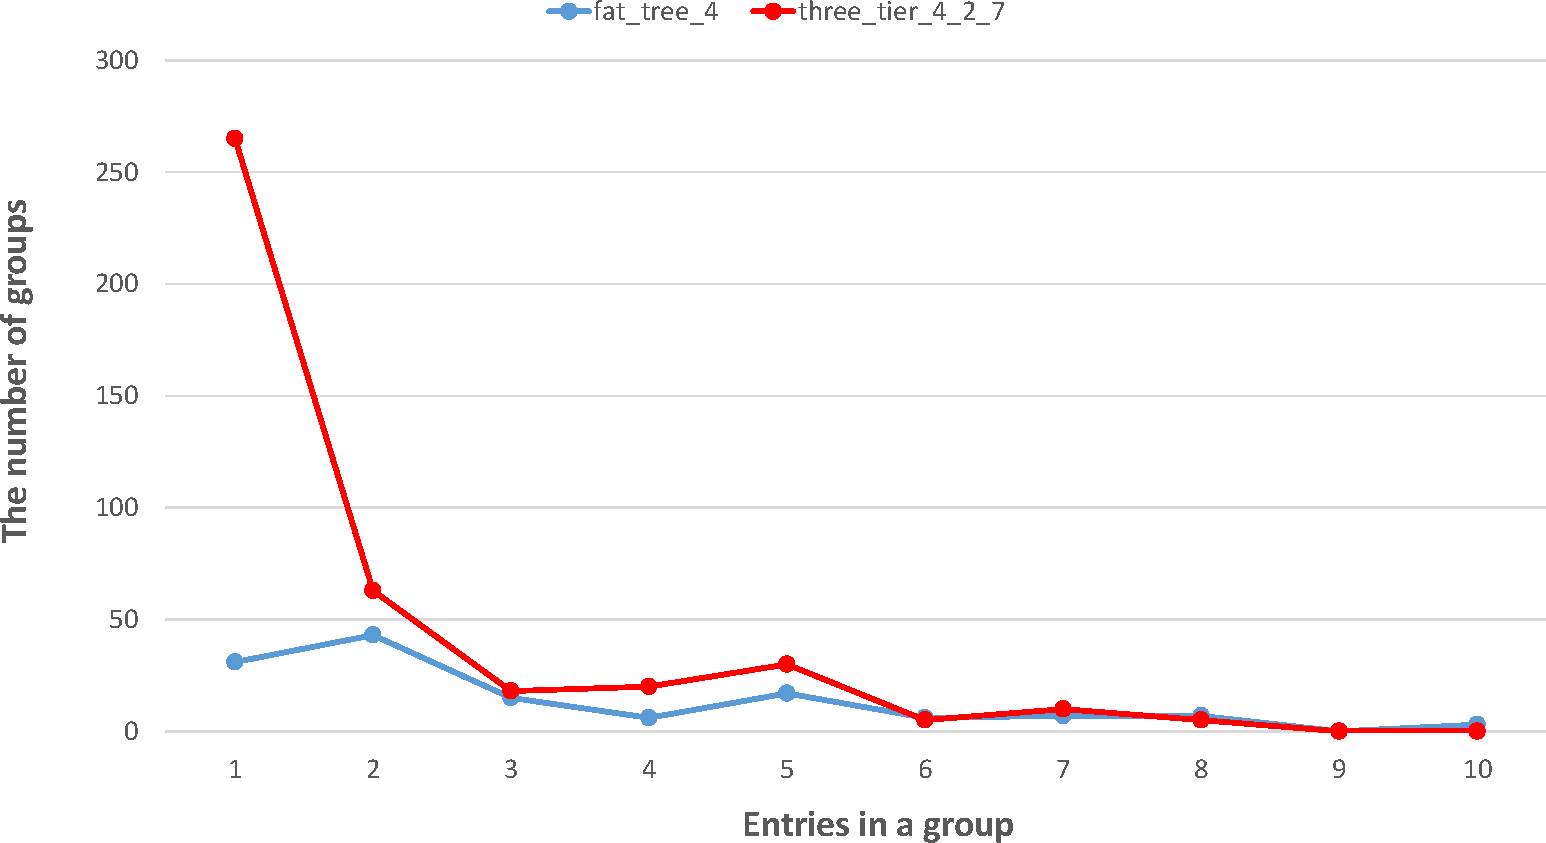
\includegraphics[width=1\linewidth]{figures/exp_topotype_distribute.pdf}
\caption{The comparison between fat\_tree\_4 and three\_tier\_4\_2\_7 -- the number of aggregated groups than contain various number of entries.}
\label{different_topo_distribute}
\end{figure}

\subsection{Influence of network scale}
To observe the influence of various network scales, different sizes of fat-tree topology will be used. Fat-tree topologies are chosen for this experiment because the other two topology types have influence on the experimental result mostly by the way switches are connected. The parameter $n$ (i.e., the number of pods) ranges from 2 to 14. Since the network scale grows significantly with a larger number of pods, we consider at most 14 pods. There are also 20 entries on each switch. The results are shown in Table~\ref{table:different_scale}, and the trend chart of effective aggregation rates and actual aggregation rates are shown in Figure~\ref{different_scale_rate_trend}.

\begin{table}
\centering
\caption{Influence of various network scales}
\begin{tabular}{|p{1.8cm}|p{1cm}|p{1.3cm}|p{1.1cm}|p{1.3cm}|}
\hline topology name & Effective aggregation rate & Actual aggregation rate & Execution time(sec) & Number of auxiliary entries \\
\hline
\hline fat\_tree\_2 & 2.70 & 2.84 & 1.26 & 35 \\
\hline fat\_tree\_4 & 2.96 & 3.27 & 8.27 & 142 \\
\hline fat\_tree\_6 & 2.85 & 3.27 & 19.16 & 327 \\
\hline fat\_tree\_8 & 2.81 & 3.29 & 33.03 & 589 \\
\hline fat\_tree\_10 & 2.91 & 3.37 & 51.81 & 921 \\
\hline fat\_tree\_12 & 2.89 & 3.36 & 74.78 & 1334 \\
\hline fat\_tree\_14 & 2.79 & 3.29 & 102.56 & 1800 \\
\hline
\end{tabular}
\label{table:different_scale}
\end{table}

In the trend chart of effective and actual aggregation rates in Figure~\ref{different_scale_rate_trend}, the aggregation rates are similar in various sizes of topology except fat\_tree\_2 which has lower aggregation rates due to fewer number of links, and the scale does not have any clear effect on the aggregation rates. Theoretically, there should be positive and negative factors that will influence the aggregation rates. The result shows that these factors break even, and the effectiveness of our method will not drop with the increasing topology size on common topology type.

\begin{figure}[ht]
\centering
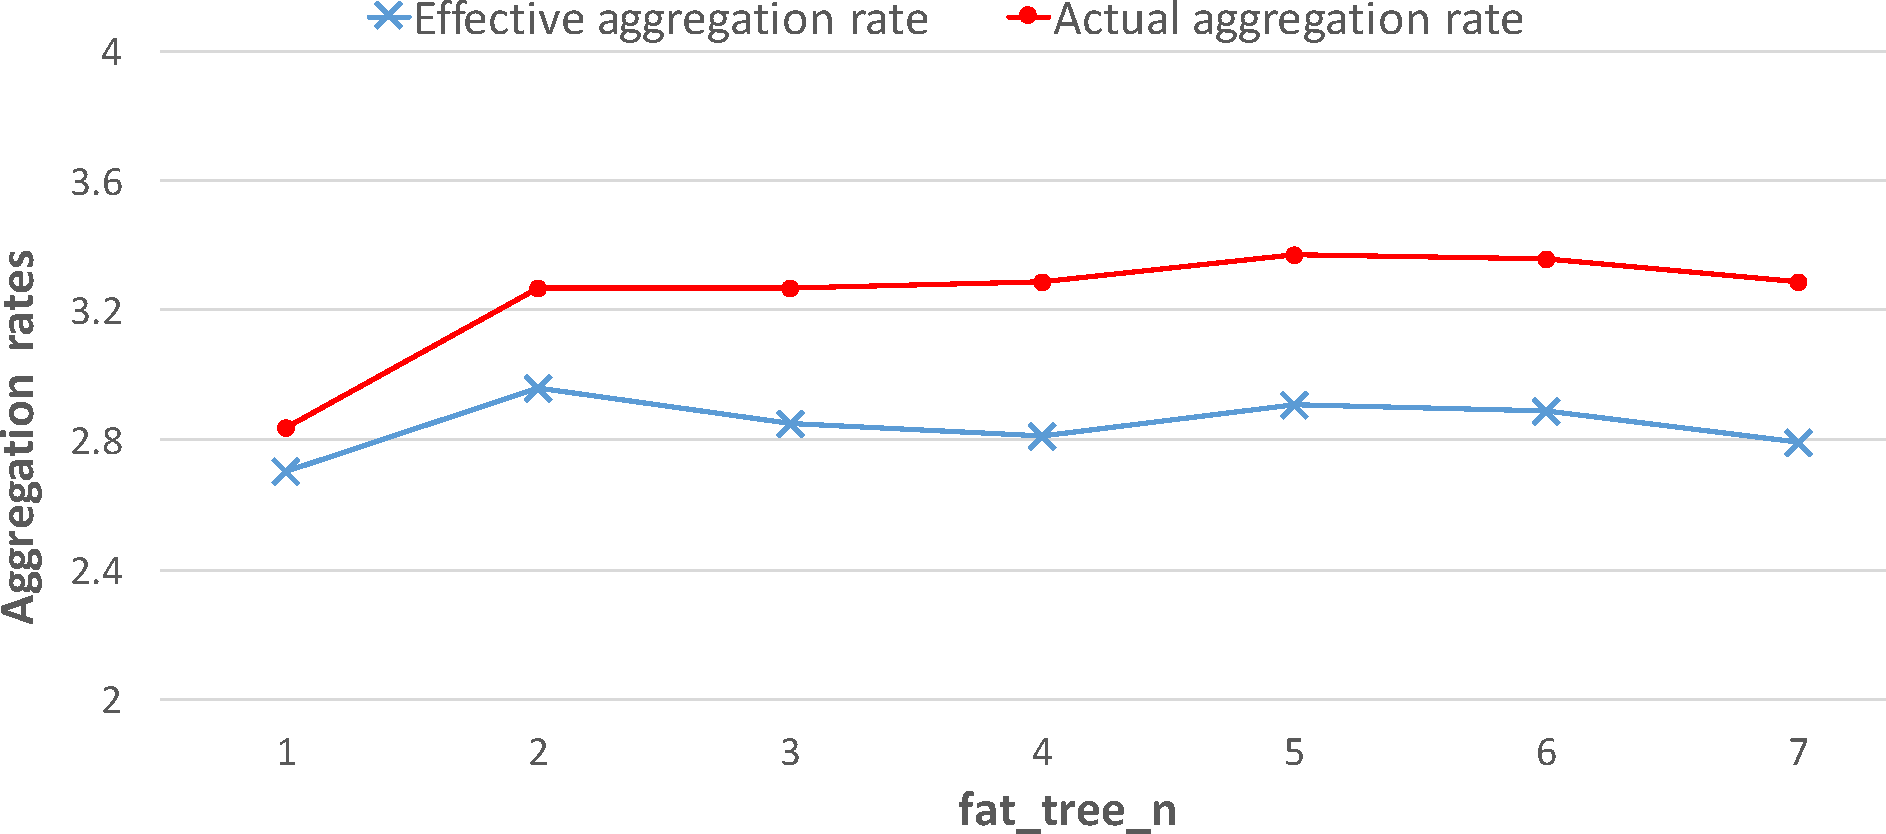
\includegraphics[width=1\linewidth]{figures/exp_scale_rate_trend.pdf}
\caption{The trend chart of aggregation rates under various scales of network.}
\label{different_scale_rate_trend}
\end{figure}

The relation between the topology size and the execution time are pretty similar, they are both proportional to $n^2$. It is quite as expected since the growth rate of switch is also proportional to $n^2$.

\subsection{Influence of flow entry number on each switch}
In this experiment, we will use fat\_tree\_4, and change the number of entries on each switch to see the influence it may bring. The number of entries on each switch increases from 10 to 200, and the intervals of entry number on each switch between every run increase as the number of entries on each switch grows. The trend chart of effective aggregation rate with various number of entries on each switch is shown in Figure~\ref{exp_entrynum_trend}. The execution time and the number of auxiliary entries grow roughly linearly along with the number of entries on a switch.

\begin{table}
\centering
\caption{Aggregation rates, execution time and number of auxiliary entries for various number of entries on a switch.}
\begin{tabular}{|p{1.8cm}|p{1cm}|p{1.3cm}|p{1.1cm}|p{1.3cm}|}
\hline Number of entries per switch & Effective aggregation rate & Actual aggregation rate & Execution time (sec) & Number of auxiliary entry \\
\hline
\hline 10 & 2.38 & 3.15 & 3.98 & 72 \\
\hline 20 & 2.96 & 3.27 & 8.27 & 142 \\
\hline 30 & 3.01 & 3.64 & 15.03 & 214 \\
\hline 40 & 3.04 & 4.03 & 19.24 & 280 \\
\hline 50 & 3.18 & 4.22 & 26.19 & 346 \\
\hline 65 & 3.35 & 4.45 & 34.31 & 461 \\
\hline 80 & 3.41 & 4.51 & 41.47 & 560 \\
\hline 100 & 3.43 & 4.47 & 55.58 & 672 \\
\hline 120 & 3.48 & 4.45 & 64.96 & 812 \\
\hline 160 & 3.60 & 4.69 & 89.21 & 1070 \\
\hline 200 & 3.60 & 4.62 & 119.47 & 1359 \\
\hline 
\end{tabular}
\label{table:different_entry_per_switch}
\end{table}

\begin{figure}[ht]
\centering
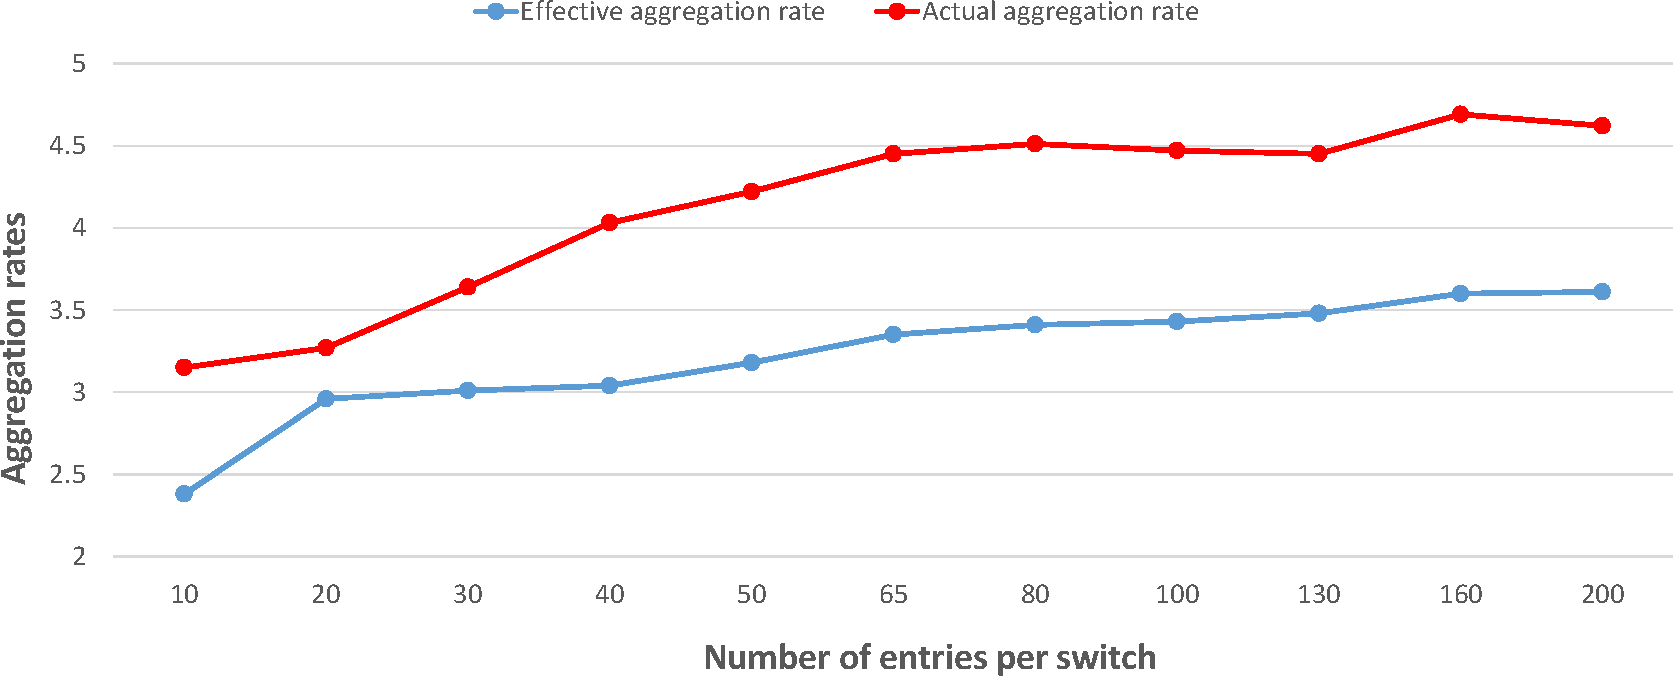
\includegraphics[width=1\linewidth]{figures/exp_entrynum_trend.pdf}
\caption{The trend chart of effective aggregation rate and actual aggregation rate with various number of entries per switch.}
\label{exp_entrynum_trend}
\end{figure}

From the trend chart in Figure~\ref{exp_entrynum_trend}, we can clearly see that the aggregation rates grow as the number of entries in the switch increases from 5 to 50 entries per switch. However, the growth rate decreases as the number of entries gets larger. A reasonable explanation is the limited number of fields in a detection packet. Two fields can be selected at each L2/L3/L4 layer at most, and a detection packet is able to accommodate no more than 6 fields and values. Hence, it is harder to find next entry that fit in the aggregated group if there are more entries in the group.

\section{Conclusion}
\label{conclusion}
We discussed the hazard that a compromised switch in SDN may bring and propose an effective way to scan  for disobedient forwarding behavior. The method detects through all the entries in topology ``fat\_tree\_4'' with around 135 packets. Also, the scale of the network topology chosen in our experiment does not affect the efficiency significantly. Last but not the least, the more entries there are in the switches, the higher aggregation rates will be; but as the effective aggregation rate get higher, it grows slower. In future work, the core algorithm can be improved by adding heuristics. Also, more realistic situation such as wildcard and multiple match fields should be considered.

% conference papers do not normally have an appendix
% use section* for acknowledgment
%\section*{Acknowledgment}


%The authors would like to thank...

% trigger a \newpage just before the given reference
% number - used to balance the columns on the last page
% adjust value as needed - may need to be readjusted if
% the document is modified later
%\IEEEtriggeratref{8}
% The "triggered" command can be changed if desired:
%\IEEEtriggercmd{\enlargethispage{-5in}}

% references section

% can use a bibliography generated by BibTeX as a .bbl file
% BibTeX documentation can be easily obtained at:
% http://mirror.ctan.org/biblio/bibtex/contrib/doc/
% The IEEEtran BibTeX style support page is at:
% http://www.michaelshell.org/tex/ieeetran/bibtex/
%\bibliographystyle{IEEEtran}
% argument is your BibTeX string definitions and bibliography database(s)
%\bibliography{IEEEabrv,../bib/paper}
%
% <OR> manually copy in the resultant .bbl file
% set second argument of \begin to the number of references
% (used to reserve space for the reference number labels box)
\begin{thebibliography}{1}

\bibitem{SOS13}
S. Scott-Hayward, G. O’Callaghan and S. Sezer,
``SDN Security: A Survey,'' In Proc. of IEEE SDN for Future Networks and Services (SDN4FNS), pp. 1–7., Nov. 2013.

\bibitem{HXWG15}
S. Hong, L. Xu, H. Wang and G. Gu,
``Poisoning Network Visibility in Software-Defined Networks: New Attacks and Countermeasures,''  In Proceedings of the 22th Annual Network and Distributed System Security Symposium (NDSS), Feb. 2015.

\bibitem{CKGL15}
P. W. Chi, C. T. Kuo, J. W. Guo and C. L. Lei,
``How to Detect a Compromised SDN Switch,'' In Proc. of the 1st IEEE Conference Network of Softwarization (NetSoft), pp. 1-6., Apr. 2015.

\bibitem{PJL16}
C. Pang, Y. Jiang and Q. Li,
``FADE: Detecting Forwarding Anomaly in Software-Defined Networks,'' In Proc. IEEE International Conference of Communications (ICC), May. 2016.

\bibitem{ZKVM12}
H. Zengyz, P. Kazemianyz, G. Varghese and N. McKeowny,
``Automatic Test Packet Generation,'' In Proc. of the 8th International Conference on Emerging Networking Experiments and Technologies (CoNEXT), Dec. 2012.

\bibitem{LAB14}
L. Schehlmann, A. Sebastian, and B. Harald, 
``Blessing or curse? Revisiting security aspects of Software-Defined Networking,'' In Proc. of 10th IEEE International Conference on Network and Service Management (CNSM), Nov. 2014.

\bibitem{KJK}
A. Khandelwal, N. Jain and S. Kamara,
``Attacking Data Center Networks from the Inside,'' \url{https://www.microsoft.com/en-us/research/wp-content/uploads/2016/02/dcn.pdf}.
 
\bibitem{AAS14}
M. Antikainen, T. Aura, and M. Särelä,
``Spook in Your Network: Attacking an SDN with a Compromised OpenFlow Switch,'' In Proc. of Nordic Conference on Secure IT System (NordSec), Oct. 2014.

\bibitem{ARDC14}
K. Agarwal, E. Rozner, C. Dixon, J. Carter,
``SDN traceroute: Tracing SDN Forwarding without Changing Network Behavior,'' In Proc. of the 3rd ACM Workshop on HotTopics in Software Defined Networking (HotSDN), Aug. 2014.

\bibitem{BCKK15}
R. Bifulco, H. Cui, G. O. Karame, F. Klaedtke,
``Fingerprinting software-defined networks,'' In Proc. of 2015 IEEE 23rd International Conference on Network Protocols (ICNP), Nov. 2015.

\end{thebibliography}

\end{document}